\documentclass{standalone}
\usepackage{tikz}
%\usetikzlibrary{...}
\begin{document}
\begin{tikzpicture}
\node at (0,0) {
   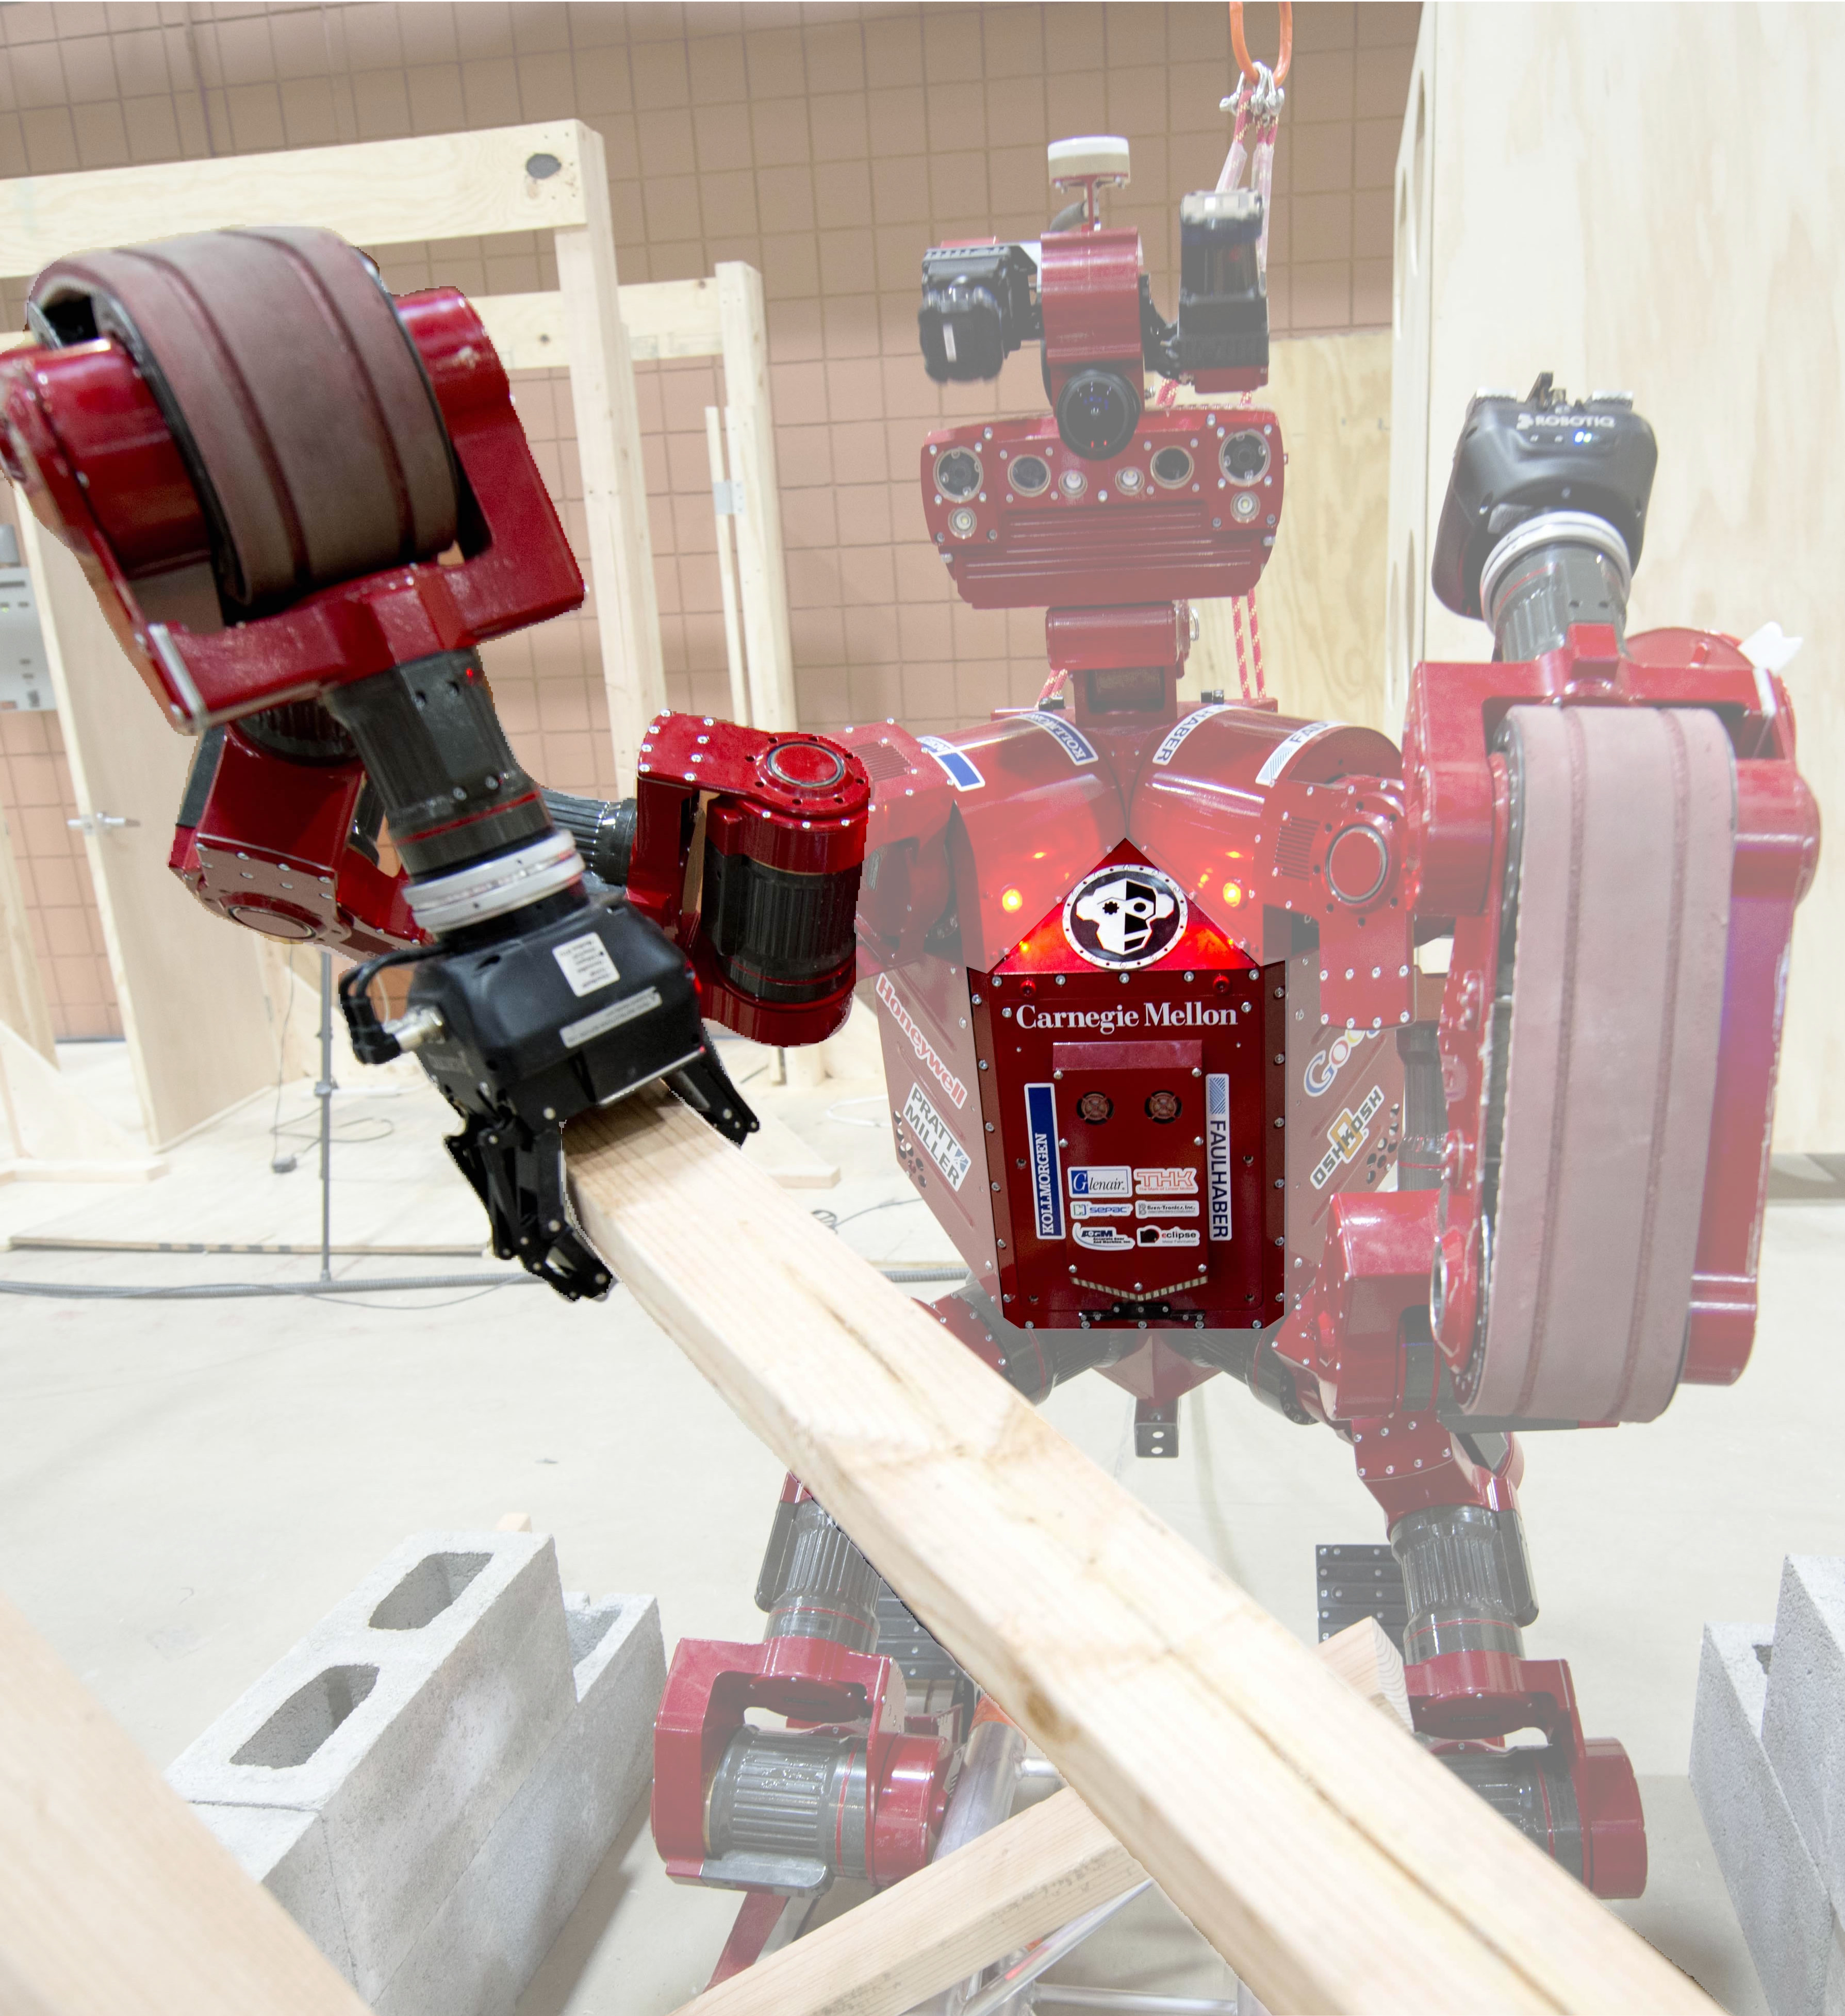
\includegraphics[height=2in]{figs/chimp-debris-cost.jpg}
};
\node[black,fill=white,fill opacity=0.5,text opacity=1]
   (planlab) at (1.0,2.15) {Planning Cost};
\draw[->,thick] (planlab.south) -- (0.6,0.6);
\node[black,fill=white,fill opacity=0.5,text opacity=1]
   (execlab) at (-0.9,-2.2) {Execution Cost};
\draw[->,thick] (execlab.north) -- (-1.1,-0.8);
\end{tikzpicture}%
\end{document}
